Da Elektronen in der Luft mit den Gasmolekülen wechselwirken, ist die Messung
\begin{wrapfigure}{r}{4cm}
  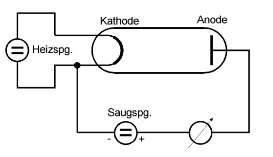
\includegraphics[width=4cm]{bilder/aufbau.jpg}
  \caption{Aufbau der Hochvakuumdiode. \cite{504}}
  \label{aufbau}
\end{wrapfigure}
des Sättigungsstroms der Elektronen nur im Vakuum möglich.
Die Elektronen werden durch ein zusätzliches elektrisches Feld vom Metall abgesaugt.
Um alle Voraussetzungen zu erfüllen, wird eine Hochvakuumdiode, wie in
Abbildung \ref{aufbau} zu sehen, verwendet.

Die Glühkathode wird durch eine Heizspannung erhitzt. Das hat zur Folge, dass
Elektronen austreten. Die gegenüberliegende Anode saugt die Elektronen über eine
Spannung $U$ ab.
Mittels Schaltung \ref{schaltA} wird der Anodenstrom $I_\su{A}$ für fünf
Heizströme $I_\su{f}$ in Abhängigkeit der Anodenspannung $U$ gemessen. Die Heizströme
liegen hierbei zwischen $2-3\Amp$.

Die Gültigkeit des Langmuir-Schottkyschen Raumladungsgebiets wird anschließend
für eine maximale Heizspannung von $3\Volt$ überprüft. Das Anlaufstromgebiet wird
für die selbe Spannung überprüft. Hierfür wird die Schaltung aus Abbildung \ref{schaltB}
verwendet
\begin{figure}
  \centering
  \begin{subfigure}{0.45\textwidth}
    \centering
    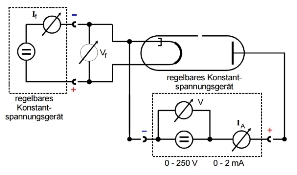
\includegraphics[width=5cm]{bilder/schaltA.jpg}
    \caption{Schaltung zur Aufnahme der Kennlinie. \cite{504}}
    \label{schaltA}
  \end{subfigure}
  \begin{subfigure}{0.45\textwidth}
    \centering
    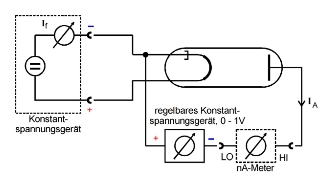
\includegraphics[width=5cm]{bilder/schaltB.jpg}
    \caption{Schaltung zur Aufnahme des Anlaufstromgebiets. \cite{504}}
    \label{schaltB}
  \end{subfigure}
\end{figure}
Das Kabel zwischen Anode und Eingangsbuchse sollte aufgrund der Störanfälligkeit
und den kleinen auftretenden Strömen möglichst kurz sein. Zusätlich kann am
Übergangswiderstand, am Heizdraht und am Nanoamperemeter ein Spannungsabfall
von mehreren Volt erzeugt werden. Dies kann dazu führen, dass die angezeigte Spannung verfälscht
wird.
Abschließend wird die Kathodentemperatur und die Austrittsarbeit ermittelt,
indem der Anodenstrom in Abhängigkeit der Anodenspannung gemessen wird.
